\section{eo\-Simple\-EDA$<$ EOT $>$ Class Template Reference}
\label{classeo_simple_e_d_a}\index{eoSimpleEDA@{eoSimpleEDA}}
eo\-Simple\-EDA: a very simple Estimation of Distribution Algorithm  


{\tt \#include $<$eo\-Simple\-EDA.h$>$}

Inheritance diagram for eo\-Simple\-EDA$<$ EOT $>$::\begin{figure}[H]
\begin{center}
\leavevmode
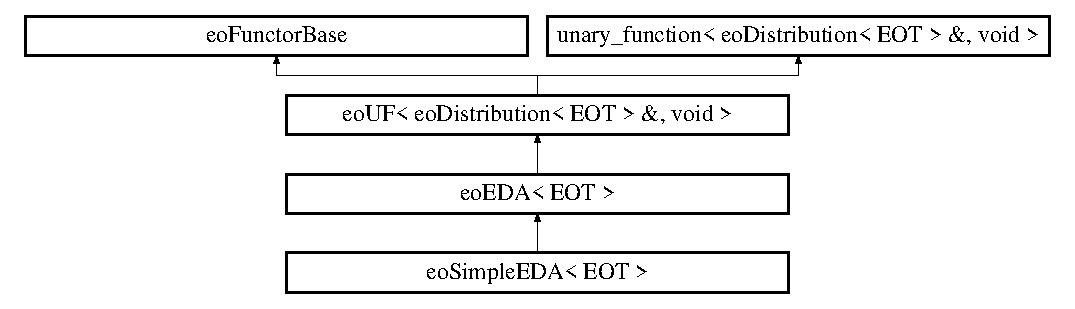
\includegraphics[height=3.70861cm]{classeo_simple_e_d_a}
\end{center}
\end{figure}
\subsection*{Public Member Functions}
\begin{CompactItemize}
\item 
{\bf eo\-Simple\-EDA} ({\bf eo\-Distrib\-Updater}$<$ {\bf EOT} $>$ \&\_\-update, {\bf eo\-Eval\-Func}$<$ {\bf EOT} $>$ \&\_\-eval, unsigned \_\-pop\-Size, {\bf eo\-Continue}$<$ {\bf EOT} $>$ \&\_\-continuator)
\begin{CompactList}\small\item\em Ctor from an {\bf eo\-Distrib\-Updater}{\rm (p.\,\pageref{classeo_distrib_updater})} ... \item\end{CompactList}\item 
virtual void {\bf operator()} ({\bf eo\-Distribution}$<$ {\bf EOT} $>$ \&\_\-distrib)\label{classeo_simple_e_d_a_a1}

\begin{CompactList}\small\item\em The algorithm: generate pop from distrib, evaluate pop, update distrib. \item\end{CompactList}\end{CompactItemize}
\subsection*{Private Attributes}
\begin{CompactItemize}
\item 
{\bf eo\-Distrib\-Updater}$<$ {\bf EOT} $>$ \& {\bf update}\label{classeo_simple_e_d_a_r0}

\item 
{\bf eo\-Eval\-Func}$<$ {\bf EOT} $>$ \& {\bf eval}\label{classeo_simple_e_d_a_r1}

\item 
unsigned {\bf pop\-Size}\label{classeo_simple_e_d_a_r2}

\item 
{\bf eo\-Continue}$<$ {\bf EOT} $>$ \& {\bf continuator}\label{classeo_simple_e_d_a_r3}

\end{CompactItemize}


\subsection{Detailed Description}
\subsubsection*{template$<$class EOT$>$ class eo\-Simple\-EDA$<$ EOT $>$}

eo\-Simple\-EDA: a very simple Estimation of Distribution Algorithm 

The algorithm that evolves a probability distribution on the spaces of populations with the loop generate a population from the current distribution evaluate that population update the distribution 



Definition at line 46 of file eo\-Simple\-EDA.h.

\subsection{Constructor \& Destructor Documentation}
\index{eoSimpleEDA@{eo\-Simple\-EDA}!eoSimpleEDA@{eoSimpleEDA}}
\index{eoSimpleEDA@{eoSimpleEDA}!eoSimpleEDA@{eo\-Simple\-EDA}}
\subsubsection{\setlength{\rightskip}{0pt plus 5cm}template$<$class EOT$>$ {\bf eo\-Simple\-EDA}$<$ {\bf EOT} $>$::{\bf eo\-Simple\-EDA} ({\bf eo\-Distrib\-Updater}$<$ {\bf EOT} $>$ \& {\em \_\-update}, {\bf eo\-Eval\-Func}$<$ {\bf EOT} $>$ \& {\em \_\-eval}, unsigned {\em \_\-pop\-Size}, {\bf eo\-Continue}$<$ {\bf EOT} $>$ \& {\em \_\-continuator})\hspace{0.3cm}{\tt  [inline]}}\label{classeo_simple_e_d_a_a0}


Ctor from an {\bf eo\-Distrib\-Updater}{\rm (p.\,\pageref{classeo_distrib_updater})} ... 

plus an eo\-Eval and {\bf eo\-Continue}{\rm (p.\,\pageref{classeo_continue})} of course 

Definition at line 53 of file eo\-Simple\-EDA.h.

The documentation for this class was generated from the following file:\begin{CompactItemize}
\item 
eo\-Simple\-EDA.h\end{CompactItemize}
